% !TeX root = ../../Book3.tex
% 纲要标题：### 23.1 Plateau 问题的竞争类
% 纲要位置：几何学计划纲要.md，第 3075 行。
% 正文状态：初稿；尚未正式审核。

% 纲要内容开始
% 
% * 边界流、竞争类和非空性
% * 锥构造与初始填充
% * 凸投影控制支集
% * 极小化序列及质量界
% 
% 纲要内容结束

\section{Plateau 问题的竞争类}
\label{g3:sec:2301}
固定一条空间闭曲线后，“寻找面积最小的曲面”还没有指定一个变分问题：允许哪些曲面，怎样理解边界，是否固定拓扑类型，都需要说明。这里用整数流记录取向、重数与边界，用质量作为面积。第22章已经给出这个类的紧性；本节补上竞争类非空以及极小化序列不向无穷远逃逸的条件。

\subsection{边界流、竞争类和非空性}
\label{g3:subsec:2301:01}
设 \(1\le k\le n\)，给定紧支整数 \((k-1)\) 流 \(B\in\mathcal I_{k-1}(\mathbb R^n)\)。我们寻找满足 \(\partial T=B\) 的整数 \(k\) 流。下标 \(k\) 是待求对象的维数；通常的空间曲线张成曲面问题对应 \(k=2,n=3\)。

\begin{definition}\label{g3:def:plateau-competitor-class}
	对紧支 \(B\in\mathcal I_{k-1}(\mathbb R^n)\)，定义竞争类及其质量下确界
	\begin{equation}\label{g3:eq:plateau-competitor-class}
		\mathcal A(B)=\{T\in\mathcal I_k(\mathbb R^n):\partial T=B\},
		\qquad m(B)=\inf_{T\in\mathcal A(B)}\mathbf M(T).
	\end{equation}
	空类的下确界约定为 \(+\infty\)。若 \(\mathcal A(B)\ne\varnothing\)，称 \(B\) 可填充。求取达到 \(m(B)\) 的元素，称为这里的\term[zhengshu liu Plateau wenti]{整数流 Plateau 问题}[integral-current Plateau problem]。
\end{definition}

\(\mathcal I_k\) 已要求流及其边界的总质量有限。因此所有竞争者都满足 \(\mathbf M(T)<\infty\)，且边界质量固定为 \(\mathbf M(B)\)。定义暂不要求竞争者紧支；允许的拓扑类型、连通分支数和整数重数也未另加限制。若把“参数域为一个圆盘”或“承载集必须连通”写入定义，得到的便是另一个竞争类，需要另行证明它在所选收敛下保持。

\begin{proposition}\label{g3:prop:euclidean-fillability}
	设 \(1\le k\le n\)，\(B\in\mathcal I_{k-1}(\mathbb R^n)\) 紧支。若 \(k\ge2\)，则 \(\mathcal A(B)\ne\varnothing\) 当且仅当 \(\partial B=0\)。若 \(k=1\)，则 \(\mathcal A(B)\ne\varnothing\) 当且仅当 \(B(1)=0\)，其中 \(B(1)\) 表示有限个带整数权点的总系数。在这两种情形下，非空类中都有紧支元素。
\end{proposition}
\begin{proof}
	如果 \(B=\partial T\)，则 \(\partial B=\partial^2T=0\)。对 \(k=1\)，这一条件对零流自动成立，还需检验总系数。取 \(\chi_R\in C_c^\infty(\mathbb R^n)\)，在 \(B_R(0)\) 上为一、支于 \(B_{2R}(0)\)，且 \(|\mathrm d\chi_R|\le C/R\)。当 \(R\) 足够大时，
	\[
		|B(1)|=|B(\chi_R)|=|T(\mathrm d\chi_R)|
		\le (C/R)\mathbf M(T)\longrightarrow0.
	\]
	故即使竞争者没有紧支集，仍有 \(B(1)=0\)。

	反过来，固定 \(a\in\mathbb R^n\)，对 \(B\) 使用\cref{g3:prop:current-cone-filling}。当 \(k\ge2\) 时，\(B\) 的维数为正，常值推前为零，而 \(\partial B=0\)，所以 \(\partial(a*B)=B\)。当 \(k=1\) 时，锥公式中的顶点项为 \(B(1)\delta_a=0\)，结论相同。锥是紧支整数流，因而属于 \(\mathcal A(B)\)。
\end{proof}

例如 \(\delta_b-\delta_a\) 可以由从 \(a\) 到 \(b\) 的有向线段填充，\(\delta_b\) 则不能成为有限质量一维整数流的边界。对高一维的边界，\(\partial B=0\) 要求每个接缝处的有向边界系数抵消；一条有两个不同端点的有向弧因而不能单独作为二维流的完整边界。

\subsection{锥构造与初始填充}
\label{g3:subsec:2301:02}
锥给出的首先是非空性与一个上界，不保证最小。若 \(B\) 满足前一命题的条件，\(\operatorname{spt}B\subset\overline B(a,R)\)，令
\[
	T_0=a*B=F_\#(\lBrack0,1\rBrack\times B),\qquad
	F(t,x)=a+t(x-a).
\]
\cref{g3:prop:current-cone-filling}给出
\begin{equation}\label{g3:eq:plateau-cone-upper-bound}
	\partial T_0=B,\qquad
	\mathbf M(T_0)\le\frac1k\int|x-a|\,\mathrm d\|B\|(x)
	\le\frac Rk\mathbf M(B).
\end{equation}
这里分母是填充维数 \(k\)。如果已经知道一个更小的显式填充，可以直接用它代替锥来改进上界。

\begin{example}\label{g3:exm:plateau-disk-initial}
	设 \(B\) 为平面 \(\mathbb R^2\times\{0\}\subset\mathbb R^n\) 中半径 \(R\) 的逆时针圆周流。取圆心为锥顶点，得到标准定向圆盘流 \(T_0\)，且
	\[
		\mathbf M(B)=2\pi R,\qquad \mathbf M(T_0)=\pi R^2.
	\]
	若边界为 \(qB\)，\(q\in\mathbb Z\)，则 \(qT_0\) 是填充，质量为 \(|q|\pi R^2\)。后面用校准证明这些上界恰为最小值。
\end{example}

当 \(k\ge2\) 时，\cref{g3:cor:integral-cycle-isoperimetric}还给出与边界所在球半径无关的上界
\[
	m(B)\le C_{n,k}\mathbf M(B)^{k/(k-1)}.
\]
它使用的是第22章的整数闭流填充定理；指数由边界维数 \(k-1\) 与填充维数 \(k\) 决定。本章的存在性只需要 \(m(B)<\infty\)，因此锥估计已经足够。

\subsection{凸投影控制支集}
\label{g3:subsec:2301:03}
质量界并不排除把一部分竞争者移到远处。解决办法是把每个竞争者投影回包含给定边界的同一个紧凸集。这个投影可以移动流，却不移动边界，也不会增加质量。

\begin{lemma}\label{g3:lem:convex-nearest-projection}
	设 \(K\subset\mathbb R^n\) 是非空闭凸集。每个 \(x\in\mathbb R^n\) 都有唯一最近点 \(p_K(x)\in K\)，且
	\begin{equation}\label{g3:eq:convex-projection-contraction}
		|p_K(x)-p_K(y)|^2\le
		\langle p_K(x)-p_K(y),x-y\rangle.
	\end{equation}
	特别地，\(p_K\) 为 \(1\)-Lipschitz 映射，且在 \(K\) 上等于恒等映射。
\end{lemma}
\begin{proof}
	取逼近距离下确界的点列。因 \(K\) 非空，这列可限制在一个固定闭球中；闭性与有限维紧性给出极限最近点。若两个不同点 \(p,q\) 都最近，则平行四边形恒等式给出
	\[
		\left|x-\frac{p+q}{2}\right|^2
		=\frac{|x-p|^2+|x-q|^2}{2}-\frac{|p-q|^2}{4}
		<\operatorname{dist}(x,K)^2,
	\]
	与中点属于 \(K\) 矛盾。

	令 \(p=p_K(x)\)。对每个 \(z\in K\)，线段 \(p+t(z-p)\) 在 \(K\) 中。函数 \(|x-p-t(z-p)|^2\) 在 \(t=0\) 的右导数非负，故
	\[
		\langle x-p,z-p\rangle\le0.
	\]
	再令 \(q=p_K(y)\)，分别取 \(z=q\) 及 \(z=p\)，将两个不等式相加，就得到式\eqref{g3:eq:convex-projection-contraction}。最后使用 Cauchy--Schwarz 不等式；当 \(p=q\) 时结论直接成立。
\end{proof}

\begin{proposition}\label{g3:prop:plateau-convex-reduction}
	设 \(1\le k\le n\)，\(B\in\mathcal I_{k-1}(\mathbb R^n)\) 紧支且可填充，\(K\) 为包含 \(\operatorname{spt}B\) 的非空紧凸集。则对每个 \(T\in\mathcal A(B)\)，
	\[
		p_{K\#}T\in\mathcal A(B),\qquad
		\operatorname{spt}(p_{K\#}T)\subset K,\qquad
		\mathbf M(p_{K\#}T)\le\mathbf M(T).
	\]
	因此令 \(\mathcal A_K(B)=\{T\in\mathcal A(B):\operatorname{spt}T\subset K\}\)，有
	\begin{equation}\label{g3:eq:plateau-same-infimum}
		m(B)=\inf_{T\in\mathcal A_K(B)}\mathbf M(T).
	\end{equation}
\end{proposition}
\begin{proof}
	\cref{g3:lem:convex-nearest-projection}和\cref{g3:cor:normal-pushforward-finite}保证推前对有限总质量的正规流有定义，与边界相容，并满足质量不增。投影通常不是固有映射；此处使用的是有限总质量的推广，而非仅局部质量有限的固有推前版本。\cref{g3:prop:rectifiable-lipschitz-pushforward}同时用于 \(T\) 与 \(\partial T\)，保证两者的推前仍为整数可整流流。因此 \(p_{K\#}T\) 是整数流。

	由于 \(p_K\) 在 \(\operatorname{spt}B\) 上等于恒等，\(p_{K\#}B=B\)。对零流，这只是逐点固定；对正维可整流流，在每个参数片上，\(p_K\) 与恒等的限制相同，其切向微分也在几乎处处相同，故可直接代入式\eqref{g3:eq:rectifiable-pushforward-formula}。于是
	\[
		\partial(p_{K\#}T)=p_{K\#}\partial T=p_{K\#}B=B.
	\]
	支集包含于闭集 \(K\)。一方面 \(\mathcal A_K(B)\subset\mathcal A(B)\)，限制后的下确界不小于 \(m(B)\)；另一方面每个竞争者均可投影为质量不大的受限竞争者，得到反向不等式。
\end{proof}

可以取 \(K\) 为包含边界的任意闭球，也可以取
\(K=\overline{\operatorname{conv}}(\operatorname{spt}B)\)。后者在边界非空时是非空紧凸集：它闭且包含在某个固定闭球中。若 \(B=0\)，直接取 \(T=0\) 即已达到最小质量，不需要对空集取最近点投影。

\begin{figure}[htbp]
	\centering
	% !TeX root = ../Book3.tex
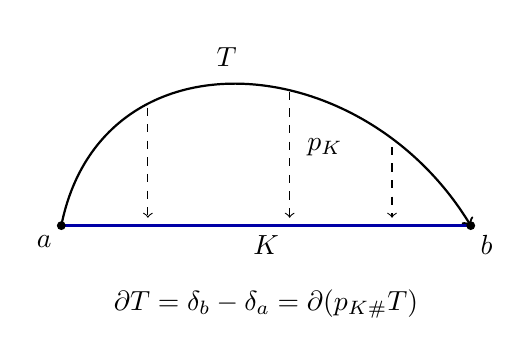
\begin{tikzpicture}[x=1cm,y=1cm]
	\draw[very thick,blue!65!black] (-2.6,0)--(2.6,0);
	\node[below] at (0,0) {\(K\)};
	\draw[thick,->] (-2.6,0) .. controls (-2.1,2.5) and (1.2,2.3) .. (2.6,0);
	\node[above] at (-0.5,1.9) {\(T\)};
	\draw[dashed,->] (-1.5,1.5)--(-1.5,0.1);
	\draw[dashed,->] (0.3,1.7)--(0.3,0.1);
	\draw[dashed,->] (1.6,1)--(1.6,0.1);
	\node[right] at (0.4,1) {\(p_K\)};
	\fill (-2.6,0) circle (1.6pt) node[below left] {\(a\)};
	\fill (2.6,0) circle (1.6pt) node[below right] {\(b\)};
	\node at (0,-1) {\(\partial T=\delta_b-\delta_a=\partial(p_{K\#}T)\)};
\end{tikzpicture}

	\caption[把竞争者投影到紧凸集]{把竞争者投影到紧凸集。图中以线段 \(K\) 和弧线示意一维情形；端点保持不动，弧线的推前落在 \(K\) 上。一般维数使用同一个 \(1\)-Lipschitz 估计控制质量。}
	\label{g3:fig:plateau-convex-projection}
\end{figure}

\subsection{极小化序列及质量界}
\label{g3:subsec:2301:04}
设 \(B\) 可填充，选定上述 \(K\)，并取一个初始竞争者 \(T_0\)。由下确界定义，对每个正整数 \(j\) 可选 \(R_j\in\mathcal A(B)\)，使
\[
	m(B)\le\mathbf M(R_j)\le m(B)+j^{-1}.
\]
令 \(T_j=p_{K\#}R_j\)。前一命题给出
\begin{equation}\label{g3:eq:plateau-minimizing-sequence}
\begin{aligned}
	&\operatorname{spt}T_j\subset K,\qquad \partial T_j=B,\\
	&m(B)\le\mathbf M(T_j)\le m(B)+j^{-1}
	\le\mathbf M(T_0)+1,\\
	&\mathbf N(T_j)=\mathbf M(T_j)+\mathbf M(B)
	\le\mathbf M(T_0)+1+\mathbf M(B).
\end{aligned}
\end{equation}
于是第22章紧性定理的全部条件已经具备：流为整数，支集共同紧，质量与边界质量有统一上界。边界质量之所以没有另外的估计困难，是因为竞争类从一开始就固定了整个边界流，而不只是边界所在的点集。

\ProseParagraphBreak
这种局部化思路见\cite[第34节，引理34.1及证明，第196--197页]{Simon1983}。这里把有限总质量但可能非紧支的竞争者也纳入比较，并显式核对投影对边界和整数性的作用。下一节从这列流出发，逐步识别极限及其质量。
% 纲要条目排为编号小节标题，并进入目录与书签；说明段仍保留于纲要注释中。
